\documentclass[crop,class=article]{standalone}
%----------------------------Preamble-------------------------------%
\usepackage{amsfonts}                   % Blackboard Bold Z.
\usepackage{tikz}                       % Drawing/graphing tools.
\usetikzlibrary{
    arrows.meta,        % Latex and Stealth arrows.
    positioning         
}
%--------------------------Main Document----------------------------%
\begin{document}
    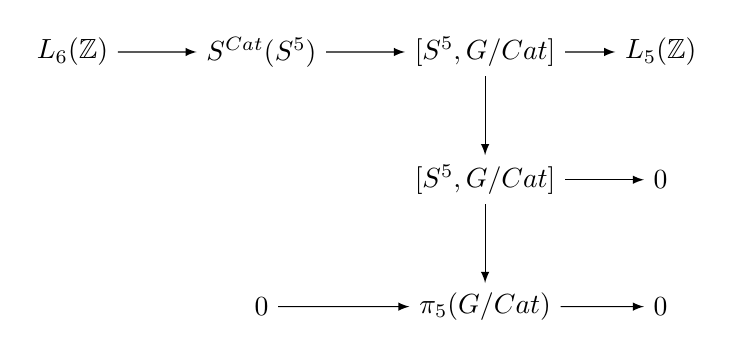
\begin{tikzpicture}[>=latex,->,scale=1.4]
        \node (a) {$[S^{5},G/Cat]$};
        \node (b) [right=of a] {$0$};
        \node (c) [below=of a] {$\pi_{5}(G/Cat)$};
        \node (d) [above=of a] {$[S^{5},G/Cat]$};
        \node (e) [left= of d] {$S^{Cat}(S^{5})$};
        \node (f) [left= of e] {$L_{6}(\mathbb{Z})$};
        \node (g) at (d -| b) {$L_{5}(\mathbb{Z})$};
        \node (h) at (c -| e) {$0$};
        \node (i) at (c -| b) {$0$};
        \path (a) edge (b);
        \path (a) edge (c);
        \path (d) edge (a);
        \path (d) edge (g);
        \path (f) edge (e);
        \path (e) edge (d);
        \path (h) edge (c);
        \path (c) edge (i);
    \end{tikzpicture}
\end{document}